\chapter{Parameter Estimation}
\ifpdf
    \graphicspath{{Chapter2/Chapter2Figs/PNG/}{Chapter2/Chapter2Figs/PDF/}{Chapter2/Chapter2Figs/}}
\else
    \graphicspath{{Chapter2/Chapter2Figs/EPS/}{Chapter2/Chapter2Figs/}}
\fi

In this study we have mainly focused on ABC methods as outlined in the previous section. The use of ABC methods arose in applications where the computation of the likelihood function,
\begin{equation}
L(\theta) = f(\mathbf{Y_{d}} | \theta),
\end{equation}
where $\mathbf{Y_{d}}$ are realisations of the data and $\theta$ is the parameter vector associated with the model, is impossible or impractical. The main theme in ABC approaches is the use of systematic comparisons between real data and simulated data to approximate the Likelihood function and therefore arrive at the desired posterior distribution,
\begin{equation}
p(\theta|\mathbf{Y_{d}}) \propto f(\mathbf{Y_{d}|\theta})\pi(\theta),
\end{equation}
where $\pi(\theta)$ is the prior distribution of parameters $\theta$. Typically simulating from $f(\mathbf{Y_{d}} | \theta)$ is straightforward. We then compare the simulated dataset $\mathbf{Y_{s}}$ with the real data $\mathbf{Y_{d}}$ and accept only those simulations where some distance metric between the two $\Delta(\mathbf{Y_{s}}, \mathbf{Y_{d}})$ falls below a certain threshold value $\epsilon$.  Generally ABC methods have the following form:
\begin{enumerate}[noitemsep]
\item{Sample a parameter vector $\theta^*$ from a proposal distribution $\pi(\theta) $}
\item{Simulate a dataset $\mathbf{Y_{s}}$ from the model characterised by conditional probability distribution $f(\mathbf{Y_{d}}|\theta)$}
\item{Compare the simulated dataset $\mathbf{Y_{s}}$ and observations $\mathbf{Y_{d}}$ according to some distance function $\mathrm{\Delta}$. If $\Delta(\mathbf{Y_{s}}, \mathbf{Y_{d}}) < \epsilon$ where $\epsilon$ is the error tolerance of accepted solutions, then accept $\theta*$ otherwise reject. }
\end{enumerate}
The output of the ABC algorithm is a sample from a distribution of the form,
\begin{equation}
p_\epsilon(\theta|\mathbf{Y_{d}}) \propto \int f(\mathbf{Y_{s}}|\theta)  (\Delta(\mathbf{Y_{d}}, \mathbf{Y_{s}} \leq \epsilon) \pi(\theta) \mathrm{d}\mathbf{Y_{s}},
\end{equation}
If the chosen value for $\epsilon$ is small enough then the obtained distribution $p_\epsilon(\theta | \mathbf{Y_{d}})$ will be a good approximation for $p(\theta | \mathbf{Y_{d}})$. Sometimes when the comparison between real and simulated datasets is difficult summary statistics of the datasets, $S(\mathbf{Y_{d}})$ and $S(\mathbf{Y_{s}})$ can be compared instead. The ABC scheme as outlined above is not very efficient in its search of the parameters space as it spends a lot of time in areas of very low likelihood where the simulated solution will no resemble the data. To this direction different computational schemes have been devised like Markov Chain Monte Carlo\cite[] {marjoram2003markov} where previous good choices advise the next choices thus creating a Markov Chain with stationary distribution the posterior and Sequential Monte Carlo methods where you sample with a decreasing $\epsilon$-schedule and from a series of distributions that increasingly resemble the target posterior\cite[] {del2006sequential, sisson2007sequential, toni2009abc}. These are the basic flavours of ABC methods although there are variants of each and these were the methods implemented and incorporated for the parameter estimation tool. In the next section there are more detailed accounts for the implemented algorithms followed by test results on 2 systems.

\section{Simple Rejection Sampler}
\label{sec:rejection_sampler}
The simpler ABC algorithm is a simple rejection sampler\cite[] {pritchard1999population} which basically follows the general form as outlined before without any modifications. It samples from a prior distribution without taking into account correct guesses and 'blindly' continues to draw samples from the prior:
\begin{enumerate}[noitemsep]
\item{Sample a parameter $\theta ^*$ from prior distribution $\pi(\theta)$.}
\item{Simulate a dataset $\mathbf{y}^*$  from model with parameters $\theta ^*$.}
\item{If $\Delta(\mathbf{Y_{s}}, \mathbf{Y}) < \epsilon$ accept $\theta^*$, otherwise reject.}
\end{enumerate}
The distance function used is a simple Euclidean distance metric,
\begin{equation}
\sum_{i=0}^{N} (\mathbf{Y_{d}}^{i} -\mathbf{Y_{s}}^{i})^2,
\end{equation}
where $\mathbf{Y_{s}}$ is the simulated dataset and $\mathbf{Y_{d}}$ is the observed dataset. This distance metric is related to traditional Maximum Likelihood Estimation subject to some assumptions and we will show that in detail in a later section. Obviously the acceptance rate for this algorithm is really low if the prior distribution is very different from the posterior since it does not take into account previous good guesses to inform the search and keeps 'blindly' jumping in parameter space. This low acceptance rate means a high number of simulation steps are needed to get a reasonable number of accepted samples to approximate the posterior and although the simulation does not have a high computational cost the number of steps needed make this algorithm a poor choice and it was just implemented as a reference point to see the improvements with the more sophisticated algorithms. Despite its obvious inefficiencies this algorithms is very simple to implement and because it has little room for tweaks since the only setting that needs tuning is the tolerance level $\epsilon$, it has little room for failure making it easy to adapt and very general. Moreover if we have some prior knowledge on the parameter values and can therefore make informed choices about the prior distributions of the parameters then the acceptance rates will not be very low. Also another charactersitic, which is common for all ABC schemes is thatthe samples are generated independently and can therefore the entire computation can be easily parallelised taking advantage of modern multi-core hardware. These characteristics can therefore make it an attractive choice for certain applications.

\section{Markov Chain Monte Carlo(MCMC)}
An improvement to the random search of the simple rejection sampler is offered by a Markov Chain Monte Carlo method in the spirit of the traditional Metropolis-Hastings algorithm but slightly modified to fit this problem\cite[] {marjoram2003markov}. The intuition behind this algorithm is that you use previous good guesses as a basis for the next sampling thereby creating a Markov Chain with stationary distribution the goal posterior:
\begin{enumerate}[noitemsep]
\item{Initialise $\theta_{i}, i = 0$.}
\item{Sample a candidate parameter vector $\theta^*$ from a proposal distribution $q(\theta^* | \theta_{i})$.}
\item{Simulate a dataset $\mathbf{y}^*$ from model with parameters $\theta^*$.}
\item{If $d(\mathbf{y}^*, \mathbf{Y}) < \epsilon$ jump to new value $\theta^*$ - making it the next value in the chain, $\theta_{i+1} = \theta^*$- with a probability given by:
\begin{equation}
a = min \left(1, \frac{\pi(\theta^*)q(\theta_{i}) | \theta^*)}{\pi(\theta_{i}q(\theta^*|\theta_{i})}\right)
\end{equation}}
\item{Set i=i+1 and continue from 2.}
\end{enumerate}
One of the decisions that was taken was to use an adaptive Gaussian distribution as a proposal distribution $q$. The proposal Gaussian from which we sample has big variance at first so that it will make big jumps in the parameter space. Once a good sample is found the variance of the proposal distribution is decreased to stay in the area. But that has the problem of getting stuck at local optimum areas for a long period of time so a rejection count is employed. If in the close vicinity we keep rejecting then the variance of the proposal distribution is increased to move out of that area. That way areas with many accepted samples are oversampled in the final population. It should be noted that univariate Gaussians were used for the proposal distributions, with each parameter in the parameter vector $\theta$ coming from a different proposal distribution. The relations between the parameters are however captured in the fact that when a sample is accepted it is accepted as whole. Despite the attempts to avoid the problem of getting stuck at local sub-optima, this algorithm is still prone to doing exactly that. One possible improvement is to change it to the original Metropolis-Hastings and therefore accepting (with low probability) samples that do not come close to the observed data. That way sometimes jumps will be made to other areas which can result in better exploration of the parameter space. This can also give a resulting population with more than one candidate value and then other criteria can be used to evaluate the fitness of the model with both set of candidate parameters. 
\section{Sequential Monte Carlo(SMC)}
\label{sec:smc}
Another variation of the ABC form is the Sequential Monte Carlo approach\cite[] {toni2009abc} which combines the common ABC algorithm form with a Sequential Monte Carlo approach.  In this algorithm instead of having a single $\epsilon$ value as tolerance we have an $\epsilon$ schedule of a series of decreasing values $\epsilon_T < \epsilon_{T-1} \dots < \epsilon_{1}$. We start by sampling from the prior $\pi(\theta)$ as before at algorithmic time $t=1$ with a tolerance level $\epsilon_{1}$. Then we accept or reject the generated samples with a comparison between real and simulated data in the standard ABC fashion. The population of accepted particles is therefore an approximation for $p_{\epsilon_{1}}(\mathbf{Y_{d}}|\theta)$. Then at algorithmic time $t=2$ instead of sampling again from the prior $\pi(\theta)$ we sample from the distribution obtained at the previous step $p_{\epsilon_{1}}(\mathbf{Y_{d}}|\theta)$. The new samples usually called particles are then moved in parameter space according to some distribution function usually parameterised by them. For example if we have sampled particle $\theta^*$ we can move it by sampling again a new particle $\theta^{**}$ from a normal distribution centred around $\theta^*$ and scaled to the previous population.This movement in parameter space is usually called perturbation and the distribution used to do it is called a perturbation kernel in ABC language. The perturbed particles are then accepted or rejected as before subject to new tolerance level $\epsilon_{2}$ thus creating the second population. This procedure is repeated for all all $T$ tolerance levels in the $\epsilon$-schedule therefore creating distributions \{$p_{\epsilon_{1}}(\mathbf{Y_{d}}|\theta)$,$p_{\epsilon_{2}}(\mathbf{Y_{d}}|\theta), $\dots, $p_{\epsilon_{T}}(\mathbf{Y_{d}}|\theta)$\} along the way. If the final $\epsilon_{T}$ is small enough then the final population should be a good approximation of the target posterior.  The algorithm therefore describes a particle-filtering procedure -we pass and filter a population of parameter values sampled from a prior $\pi(\theta)$  from a series of distributions with the decreasing $\epsilon$-schedule so that the intermediate distributions gradually go towards the posterior(this particle-filtering view can be better seen with Figure\ref{fig:smc}). The particular SMC algorithm that we use is from \cite[] {toni2009abc} which also uses the notion of importance sampling, assigning weights to each particle in the population and then in the next step sampling from the weighted distribution,
\begin{figure}
\centering
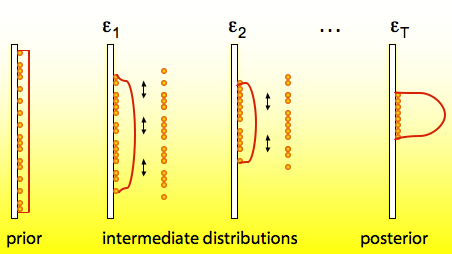
\includegraphics[width=0.5\linewidth]{ABCSMC}
\caption{In the SMC algorithm a sample from the prior distribution $\pi(\theta)$ is passed through filtering steps where the probability of the particles to represent the data best is updated during the algorithm via intermediate distributions. The final distribution $p_{\epsilon_{T}}$ is an approximation of the posterior distribution. The SMC  algorithm follows a particle-filtering approach.}
\label{fig:smc}
\end{figure}

\begin{enumerate}[noitemsep]
\item{Initialise the $\epsilon$-sequence $\epsilon_{1}, \dots, \epsilon_{T}$}
\item{If $t=0$, sample $\theta^*$ from prior $\pi(\theta)$\\
Else, sample $\theta^*$ from previous population $\theta_{t-1}^{i}$ with weights $w_{t-1}$ and perturb it with a perturbation kernel $K_{t}(\theta|\theta^*) $ to get particle $\theta^{**}$.}
\item{Simulate dataset $\mathbf{y}^*$ from model with parameters $\theta^{**}$.}
\item{if $d(\mathbf{y}^*, \mathbf{Y}) > \epsilon_{t}$ go back to 2, otherwise accept particle -set $\theta_{t}^{(i)} = \theta^{**}$- and calculate its associated weight by:
\begin{equation}
w_{t}^{(i)} = \begin{cases} 1, & \mbox{if } t\mbox{ = 0} \\ \frac{\pi(\theta_{t}^{(i)})}{\sum_{j-1}^N w_{t-1}^{(j)}K_{t}(\theta_{t-1}^{(j)}, \theta_{t}^{(i)}} , & \mbox{if } \mbox{$ t > 0$} \end{cases}
\end{equation} }
\item{Continue for all $\epsilon \in \left\{{\epsilon_{1}, \dots, \epsilon_{T}}\right\}$}
\end{enumerate}

It should be noted that in the special case where $T=1$ the algorithm reduces to the simple rejection algorithm described in section \ref{sec:rejection_sampler}.  The success of the algorithm both in computational and quality of the solution depends on the choice of the $\epsilon$ schedule and the perturbation kernel $K_{t}$. The effect of the $\epsilon$-schedule is easy to see: if two successive tolerance levels $\epsilon_{t}$ and $\epsilon_{t+1}$ are close to each other then the corresponding intermediate distributions $p_{\epsilon_{t}}(\mathbf{Y_{d}}|\theta)$ and $p_{\epsilon_{t+1}}(\mathbf{Y_{d}}|\theta)$  will be similar and therefore the acceptance rate of the filtering procedure at that step will be high with the disadvantage however that the procedure will not much progress towards the posterior.  A slowly decreasing $\epsilon$-schedule will therefore results in a high number of filtering steps(large value of $T$). On the other hand if two successive tolerance values are further apart the opposite holds: the acceptance rate will suffer but the progress of the algorithm will be faster with a lower number of iterations. Despite the easy to understand intuition determining what tolerance values are close and which ones are not depends on the application at hand. Therefore there is the danger that the algorithms completely fails with particular choices of the $\epsilon$-schedule. The common choice until recently was to manually fix the schedule of tolerance values beforehand according to the model however there have been proposals for an adaptive schedule. Although we started with a hand-tuned schedule we changed that to an adaptive choice. At step $t+1$ the choice for the tolerance level, $\epsilon_{t+1}$ at that step is based on the $a$-th quantile of the distances between the accepted simulated data $\{\mathbf{Y_{s}}^{(i,t)}\}_{1 \le i \le N}$ and real data $\mathbf{Y_{d}}$ at previous step $t$. We have found that the adaptive choice for the schedule with the correct choice of $a$ improves the efficiency of the algorithm significantly for our tests cases. However in \cite[] {silk2012optimizing} it is argued that some choices of $a$ may result in the algorithm not converging to the required posterior $p_{\epsilon}(\cdot| \theta)$ so the value of the choice of the quantile is an important one.

The second algorithm setting that affects the performance is the choice for the perturbation kernel $K_{t}$. A local perturbation kernel hardly moves the particles and therefore results in high acceptance rates in the filtering steps if the successive tolerance levels are close enough.  A perturbation kernel with higher variance spreads the search more resulting in better exploration of the parameter space but at the cost of low acceptance rates. Various perturbation kernels have been proposed, component-wise normal and uniform, multivariate normal and uniform, more local ones depending on a part of the previous population or on the local Fisher Information. In \cite[] {filippi2011optimal} they also try to find optimality criteria for these kernels. In our implementation at first a component-wise perturbation uniform kernel was used so each parameter was sampled and perturbed independently. In this case the correlation betwen the parameters is captured by the fact that they are either accepted or rejected together. The $k$-th component of parameter vector $\theta$ was perturbed with uniform kernel $\sim \mathcal{U}(\theta_{k}-\sigma_{j}^{t}, \theta_{k}+\sigma_{j}^{t})$.  We set the value for $\sigma_{j}^{t}$ to the scale of the previous population,
\begin{equation}
\sigma_{j}^{t} \approx ( \underset{1 \le j \le N}{\max}\{\theta_{k}^{t-1}\} - \underset{1 \le j \le N}{\min}\{\theta_{k}^{t-1}\}).
\end{equation} 
We have also tried multivariate kernels where each particle is perturbed according to a multivariate normal distribution with covariance matrix $\Sigma^t$ based on the previous population which captures the correlation between parameters more formally. In particular we used a local kernel based on the M nearest neighbours of the sampled particle in the previous population. This proceeds in the following way: for each sampled particle $\theta$ its M nearest neighbours from the previous population $\{ \theta^{(\i, t-1)}m 1 \le i \le N\}$ are selected and the particle is perturbed according to a multivariate Gaussian distribution with mean $\theta$ and covariance matrix the empirical covariance matrix of those M-nearest neighbours, $\Sigma_{\theta, M}^{(t)}$. The main advantage of this aproach is that generally it will lead to high acceptance rates due to the locality of the movement in parameter space however this should not be done at the cost of very small exploration of the parameter space. This is directly related to the choice of the value of $M$: too small of a choice can lead to a lack of exploraition of parameter space while too large of a choice can give no advantages over standard multivariate kernels which rely on the entire previous population. Although theoretically a combination of kernels with different values of $M$ would be a good idea, practically the value of $M$ needs to be set beforehand and this choice could be a potential problem for this algorithm.

The choice of the kernel can also affect the choice for $\alpha$ in the adaptive $\epsilon$-schedule regime. For very local kernels which do not move the particles too much an aggressive choice of $\alpha$ giving large difference between successive tolerance levels can cause the algorithm to fail. On the other hand for more spread-out kernels an aggressive choice for $\alpha$ may work well.
We provide some results in the Results section\ref{sec:results} in an attempt to compare the efficiency between the different settings of the algorithm but for a more detailed and formal treaty of the topic we refer to \cite[] {filippi2011optimal}. 
\subsection{Using Fourier Distance as a distance metric}
\label{sec:fourier}
In the work of \cite[] {konopka2010gene}, the observations for the system's variables are treated as signals and their Fourier Transforms are used as a tool for model selection. We try to use the Fourier Transform as part of the distance function $\Delta$ that is used to compare real and simulated data in the SMC algorithms in order to try and capture some qualitative features of the system in question like the shape of the functions.For example this is particularly important for applications that require the presence of oscillations. In those cases a mere reproduction of the experimental data is not enough. We created a new value called 'Fourier Distance' between real $\mathbf{Y_{d}}$ and simulated datasets $\mathbf{Y_{s}}$ defined as the average distance between the dominant components of the Fourier Transforms of the constituent signals(variables) of the two.

\section{Results}
In this section we will test the implemented algorithms on two models. For the first model we will focus on the differences between ABC flavours, rejection sampling, MCMC, SMC. For the second model we will only test the SMC algorithm and focus on the differences between different settings of the algorithm namely the choice for $\epsilon$-schedule and perturbation kernel. The second model is also chosen purposefully to illustrate some of the richness of information obtained from the SMC algorithm regarding system's dynamics and sensitivity.

\subsection{Parameter inference for the Lotka-Volterra model}
The algorithms were first tested on the simple Lotka-Volterra predator-prey system\cite[] {lotka1925elements}. It is a well studied system which consists of two coupled non-linear differential equations which correspond in the original interpretation to populations of predators and prey, 
\begin{equation}
\begin{array}{lcl}
\dot x &=& ax - xy \\
\dot y &=& bxy - y \\
\end{array}
\end{equation}
The system has two fixed points at $(0, 0)$ and $(a, 1/b)$. We are interested in the second fixed point because closed trajectories surround it in phase space corresponding to solutions which oscillate around that fixed point. We set the parameter values $(a,b) = (1,1)$ which make the second fixed point $(1, 1)$ so we set initial conditions around it $(x,y) = (1, 0.5)$ which result in oscillating solutions. We create a synthetic dataset from 8 points chosen at regular intervals in the range $[0, 15]$(for exact dataset used see Appendix). Then we add white Gaussian noise to each data point according to $\sim \mathcal{N}(0,(0.5)^2)$ to account for observational errors and make the dataset more realistic. We use the standard euclidean distance $\Delta(\{x_d, y_d\}, \{x, y\})$ between the real dataset $\{x_d[i], y_d[i]\}$ and simulated dataset $\{x[i], y[i]\}$ given as usual as the sum of squared errors between them,
\begin{equation}
\Delta(\{x_d, y_d\}, \{x, y\}) = \sum_{i}\left((x[i] - x_d[i] )^2 + (y[i]-y_d[i])^2\right).
\end{equation}
The choice for the euclidean distance comes from its relation to the likelihood function which is demonstrated in a later section(\ref{sec:likelihood}). We tested the distance between real and noisy datasets and found that averaged over many runs it is equal to $\approx 4$ so we deemed the tolerance level of $\epsilon=4.5$ as a good choice. 

We first tested with the simple rejection sampler as described in section\ref{sec:rejection_sampler}. The priors were taken to be uniform for both parameters: $a \approx \mathcal{U}(-10, 10), b \approx \mathcal{U}(-10, 10)$. In order to accept 100 particles 307816 simulation steps were needed which gives an acceptance rate of around $3 \times 10^{-4}$ which is, as expected, too low. The parameters are well inferred, $a$ : median=$1.04$, interquartile range=$0.12$, $b$: median=1.1, interquartile range=0.25 and the inferred posterior distributions, $p(a|\mathbf{Y_d})$ and $p(b|\mathbf{Y_d})$, can be seen in Figure\ref{fig:rej_posteriors_lv}.
\begin{figure}
\centering
\begin{subfigure}{.5\textwidth}
  \centering
  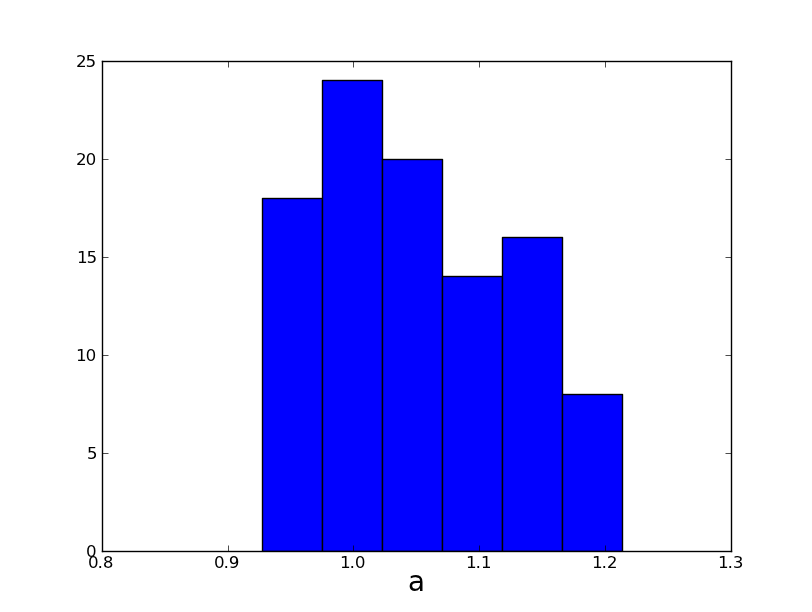
\includegraphics[width=.8\linewidth]{lv_rej_th1}
  \caption{$p_{\epsilon=4.5}(a|\mathbf{Y_d})$}
  \label{fig:sub1}
\end{subfigure}%
\begin{subfigure}{.5\textwidth}
  \centering
  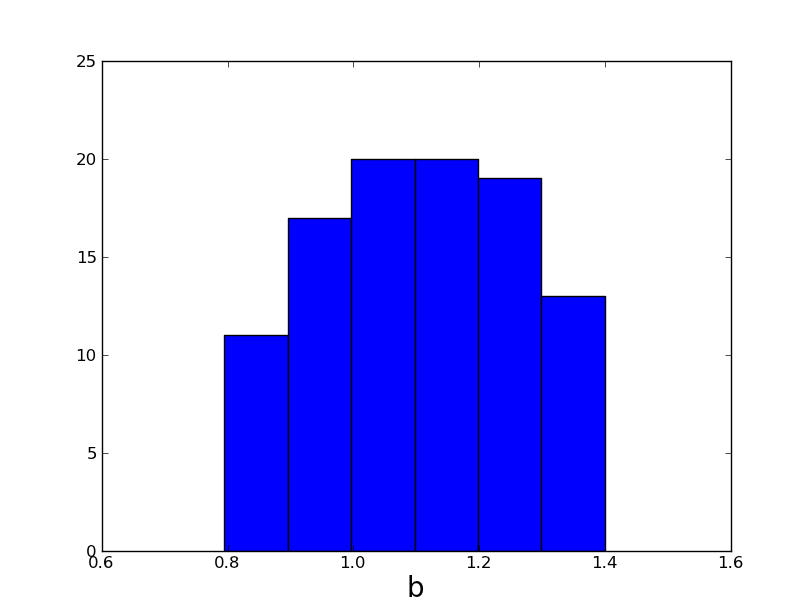
\includegraphics[width=.8\linewidth]{lv_rej_th2}
  \caption{$p_{\epsilon=4.5}(b|\mathbf{Y_d})$}
  \label{fig:sub2}
\end{subfigure}
\caption{Posteriors distributions for the two parameters $a$ and $b$ of the Lotka-Volterra model inferred with the simple rejection sampler.}
\label{fig:rej_posteriors_lv}
\end{figure}
The only setting that has to be manually adjusted for this algorithm is the tolerance level $\epsilon$ which makes it , despite its obvious inefficiencies, an attractive choice especially for applications where there are information on the parameter values beforehand and therefore the priors are close to the desired posteriors. 

We then test the SMC algorithm as described in section\ref{sec:smc} with different settings of the algorithm. Again we try to infer parameters posteriors distribution for the two parameters, $p(a|\mathbf{Y_d})$ and $p(a|\mathbf{Y_d})$. The priors for both parameters as before are set to $a \approx \mathcal{U}(-10, 10), b \approx \mathcal{U}(-10, 10)$.  We tested with a manually tuned $\epsilon$-schedule, $\{30.0, 16.0, 6.0, 5.0, 4.3\}$ and an adaptive $\epsilon$-schedule based on the 0.1-th quantile of the distances of the previous population. The perturbation kernel $K_t$ was set to a component-wise uniform one to the scale of the previous population.  For the manually tuned schedule in order to accept 100 particles in the last population $26210$ steps were needed in total over all iterations. The cumulative number of steps taken over the course of the algorithm's iterations can be seen in Table\ref{tab:dsteps_man}. The numbers verify the claims in the previous section: the big difference between $\epsilon_1$ and $\epsilon_2$ is reflected in the big number of simulation steps needed to go from $t=1$ to $t=2$. On the other hand very few simulation steps are needed in later iterations due to the small difference between the corresponding tolerance levels. The inferred posteriors in Figure\ref{fig:smc_man} agree with the values used to generate the synthetic dataset, $a$:[median=$1.04$, interquartile range=$0.13$], $b$:[median=$1.03$, interquartile range=0.32]. The quality of the solution corresponding to the inferred parameter values can also been seen in Figure\ref{fig:smc_man}. 

For the adaptive scheduled in order to accept 100 particles at the last iteration $11030$ steps were needed in total for all iterations which is half of that needed in the manually tuned schedule experiment. The adaptive choice can be more efficient but care has to be taken when choosing the value of $\alpha$ because a too aggressive choice can sometime pay off making the process more efficient but other times can cause the algorithm to get stuck and fail. The cumulative number of steps needed at each iteration can be seen in Table \ref{tab:dsteps_ad}.  We can see from the inferred posteriors and the quality of the solution(Figure \ref{fig:smc_ad}) that the estimates with the adaptive $\epsilon$-schedule are more narrow and very close to the true value. This is due to the fact that the last tolerance level is not set beforehand so if the tolerance level values have not converged at that point the algorithm can keep going with smaller tolerance values until it does. 



\begin{table}[ht]
\centering
\begin{tabular}{ l*{5} c r }
\hline
population              & 1 & 2 & 3 & 4 & 5 \\
\hline
data generation steps & 208 & 24 844 & 25735 & 25 997 &  26210   \\
\hline
\end{tabular}
\caption{Cumulative data generation steps needed for each population in the SMC algorithm using a manually tuned $\epsilon$-schedule for the Lotka-Volterra model(component-wise uniform kernel to the scale of the previous population).}
\label{tab:dsteps_man}
\end{table}

\begin{table}[ht]
\centering
\begin{tabular}{ l*{8} c r }
\hline
population              & 1 & 2 & 3 & 4 & 5 & 6 & 7 & 8 \\
\hline
data generation steps &162& 2972& 4983& 9359& 9841& 10202& 10602& 11030 \\
\hline
\end{tabular}
\caption{Cumulative data generation steps needed for each population in the SMC algorithm using an adaptive $\epsilon$-schedule based on the 0.1-th quantile of the previous population for the Lotka-Volterra model(component-wise uniform kernel to the scale of the previous population).}
\label{tab:dsteps_ad}
\end{table}

\begin{figure}[!htbp]
\def\tabularxcolumn#1{m{#1}}
\begin{tabularx}{\linewidth}{@{}cXX@{}}
%
\begin{tabular}{cc}
\subfloat[]{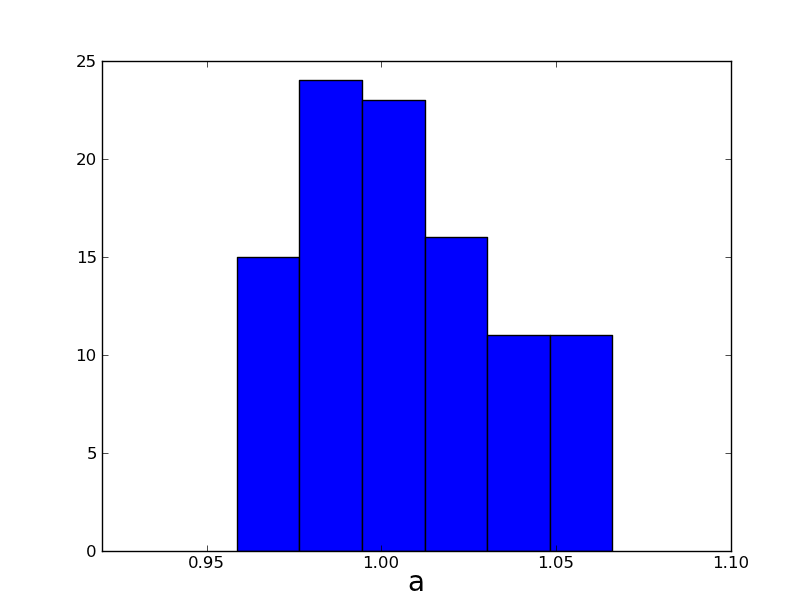
\includegraphics[width=0.5\linewidth]{smc_ad_hist_th1}} & \subfloat[]{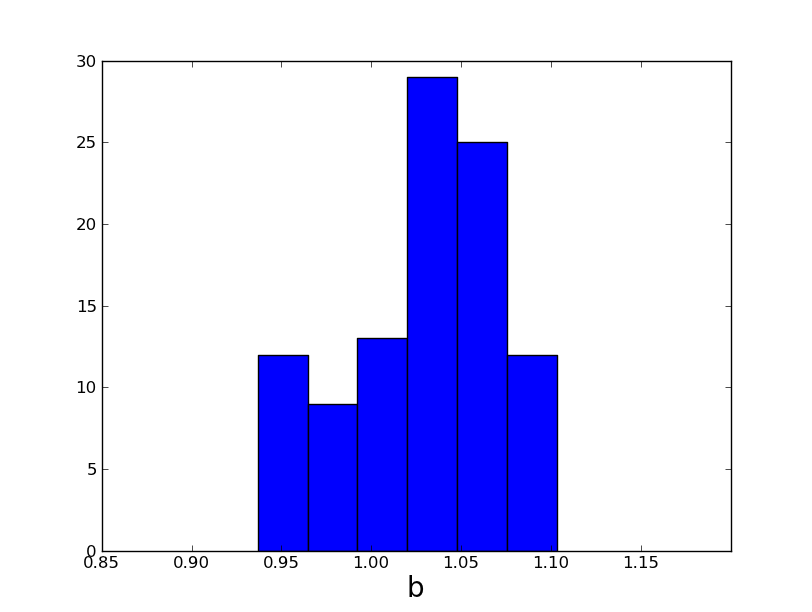
\includegraphics[width=0.5\linewidth]{smc_ad_hist_th2}}\\
\subfloat[]{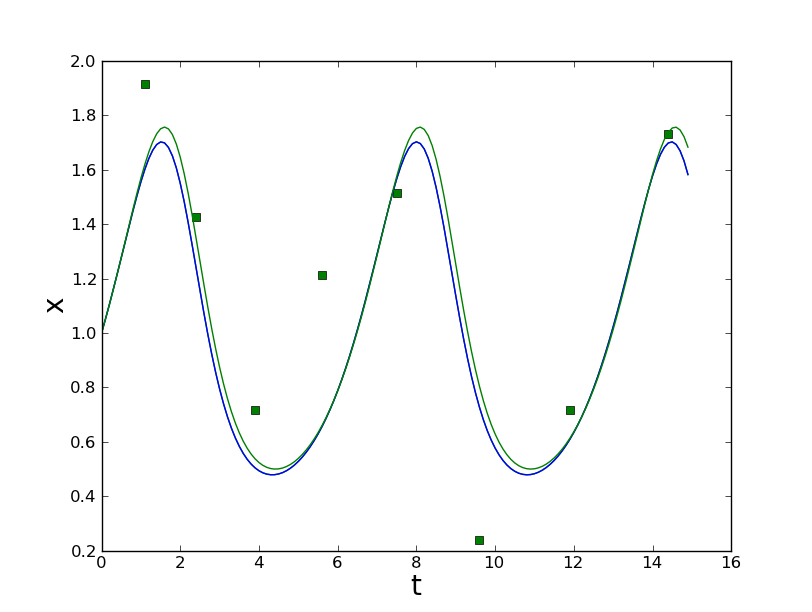
\includegraphics[width=0.5\linewidth]{smc_ad_x}} & \subfloat[]{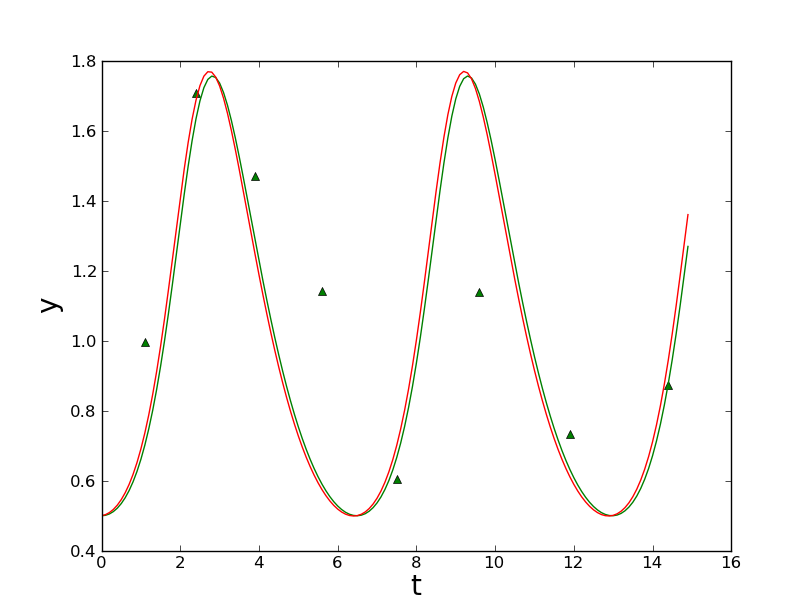
\includegraphics[width=0.5\linewidth]{smc_ad_y}}\\
\end{tabular}
\end{tabularx}
\caption{Inferred posteriors and quality of solution}\label{fig:smc_ad}
\end{figure}

\begin{figure}[!htbp]
\def\tabularxcolumn#1{m{#1}}
\begin{tabularx}{\linewidth}{@{}cXX@{}}
%
\begin{tabular}{cc}
\subfloat[]{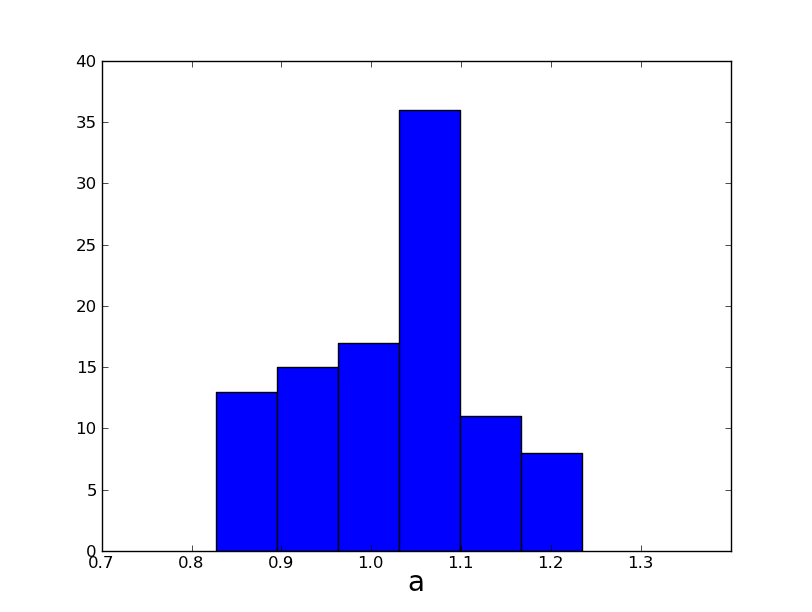
\includegraphics[width=0.5\linewidth]{smc_man_th1}} & \subfloat[]{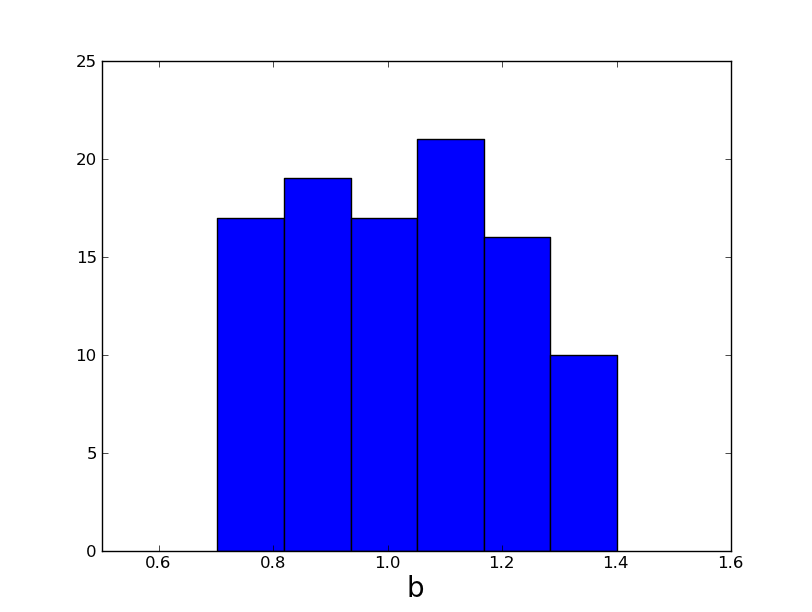
\includegraphics[width=0.5\linewidth]{smc_man_th2}}\\
\subfloat[]{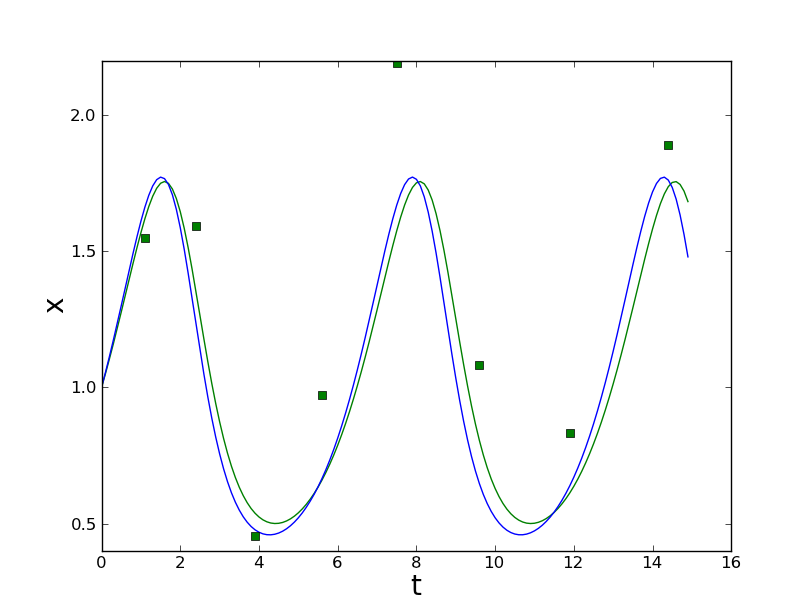
\includegraphics[width=0.5\linewidth]{smc_man_x}} & \subfloat[]{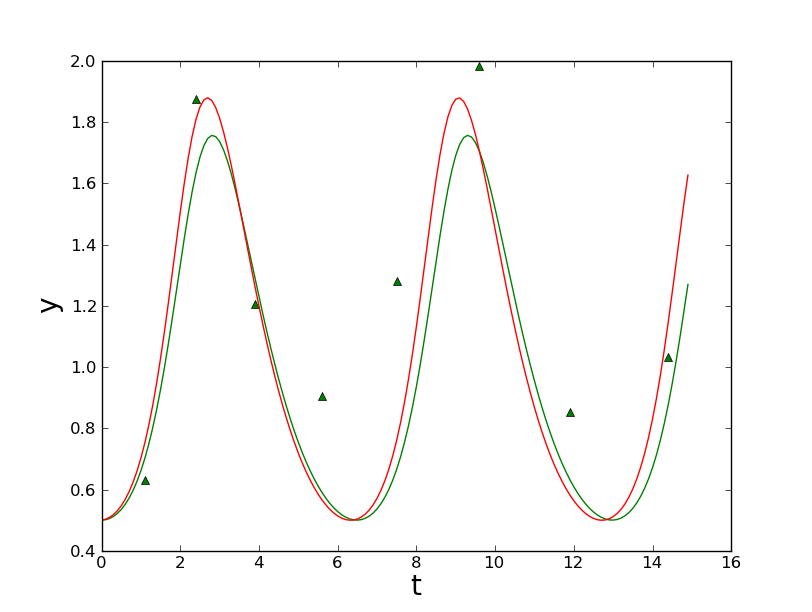
\includegraphics[width=0.5\linewidth]{smc_man_y}}\\
\end{tabular}
\end{tabularx}
\caption{Inferred posterior distributions.}\label{fig:smc_man}
\end{figure}

We also tested the algorithm with local multivariate normal kernels with an adaptive choice for the $\epsilon$-schedule as before.  The kernels are local in the sense that their covariance matrix is the empirical covariance matrix of the $M$ nearest neighbours from the previous population as explained in the previous section. For this particular example for values of $M $ less than half the size of the previous population we observed that less data generation steps are needed compared to the uniform component-wise case. The total data generation steps needed for different values of $M$ are summarised in Table \ref{tab:dsteps_multi}. As far as the inferred parameters go the results are similar to the results using the uniform kernels.

Finally we test the algorithm using the Fourier Distance metric, introduced in a previous section\ref{sec:fourier}. The number of datapoints taken in the interval of interest in previous tests to serve as the dataset in not enough in this case. In order to treat the time series as a signal and take its Fourier Transform we need more datapoints in the interval so for both the original and simulated datasets in the process we took 150 points in the range $[0, 15]$ at regular $0.1$ intervals, a number which is not realistic in practise but which we use here to demonstrate the relevance of the Fourier Distance as an adequate summary descriptor for the system in question. The results are comparable to the ones obtained before, $a$: median=$1.05$, $b$: median=$0.99$ and the kind of solution that this gives can be seen along with the noisy dataset in Figure\ref{fig:four_solution}. In most of these applications however

\begin{figure}
\centering
\begin{subfigure}{.5\textwidth}
  \centering
  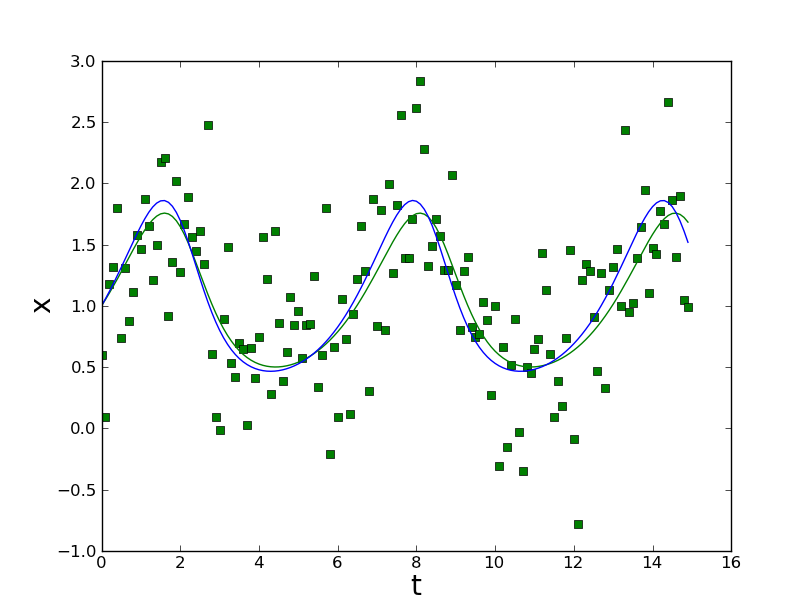
\includegraphics[width=.8\linewidth]{smc_fourier_x}
  \caption{$p_{\epsilon=4.5}(a|\mathbf{Y_d})$}
  \label{fig:sub1}
\end{subfigure}%
\begin{subfigure}{.5\textwidth}
  \centering
  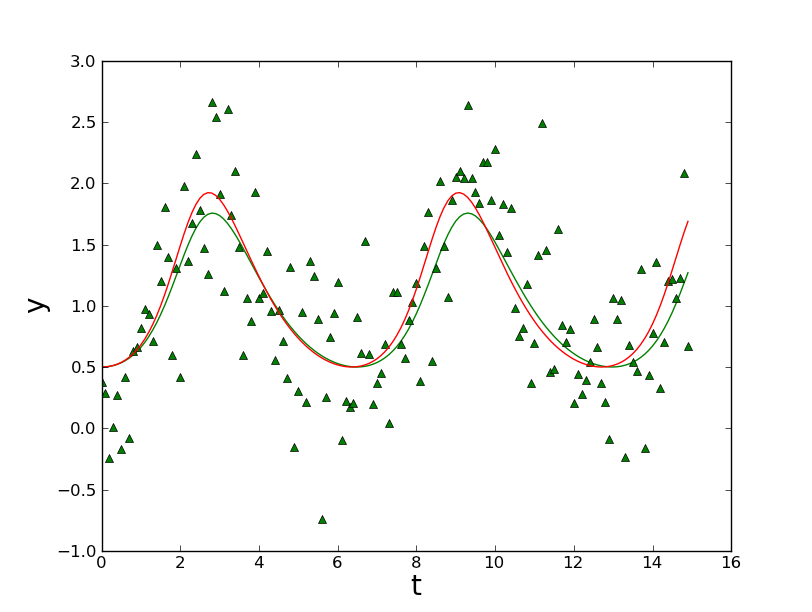
\includegraphics[width=.8\linewidth]{smc_fourier_y}
  \caption{}
  \label{fig:sub2}
\end{subfigure}
\caption{Posteriors distributions for the two parameters $a$ and $b$ of the Lotka-Volterra model inferred with the simple rejection sampler.}
\label{fig:four_solution}
\end{figure}



\subsection{Parameter inference for repressilator model}
To test the implemented SMC algorithm we turn into a molecular biology example, the repressilator model which was purposefully chosen to highlight some of the challenges associated with parameter estimation and also the utility of the information gathered from ABC algorithms. The repressilator model\cite[] {garcia2004modeling} is a popular synthetic gene regulatory network. It consists of three genes connected in a feedback loop and each of the genes transcribes for a protein that represses the next gene in the loop with the last one repressing the first(Figure\ref{fig:repressilator}). The evolution of the concentrations of the mRNA products and their corresponding proteins can be written as a system of ODEs,
\begin{equation}
\begin{array}{lcl}
\dot m_1 & = & -m1 + \frac{\alpha}{1 + p_{3}^{n}} + \alpha_0 \\
\dot p_1& = & -\beta(p_1 - m_1) \\
\dot m_2 & = & -m2 + \frac{\alpha}{1 + p_{1}^{n}} + \alpha_0 \\
\dot p_2 & = & -\beta(p_2 - m_2)\\
\dot m_3 & = & -m3 + \frac{\alpha}{1 + p_{2}^{n}} + \alpha_0 \\
\dot p_3 & = & -\beta(p_3 - m_3),
\end{array}
\end{equation} 
\begin{figure}
\centering
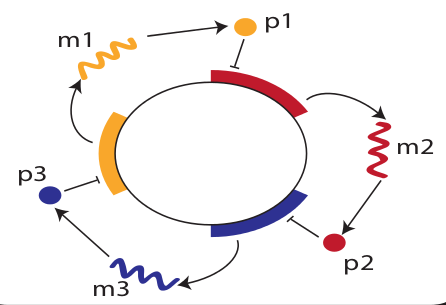
\includegraphics[width=0.5\linewidth]{repressilator}
\caption{The repressilator model. Three genes connected in a feedback loop where the protein product of each gene represses the production of the next gene in the loop.}
\label{fig:repressilator}
\end{figure}
where $m_i$ denotes the mRNA concentration and $p_i$ the corresponding protein one.  The model is parameterised by parameter vector $\theta = (\alpha, \alpha_0, \beta, n)$ where $n$ is the Hill coefficient, $\alpha$ the repression strength, $\beta$ the ratio of the protein decay rate to the mRNA decay rate and $a_0$ the basal expression rate. 

We assume that only the mRNA concentrations $\{m_i\}_1 \le i \le 3$ are known. We fix the parameter values at $(\alpha, \alpha_0, \beta, n) = (216.0, 0.216, 5.0, 2.0)$ and create a synthetic dataset consisting of the mRNA concentrations at timepoints taken at regular intervals in the range $[0, 50]$(for the exact dataset used see Appendix). We also assume that the initial condition are known: $(m_1, m_2, m_3, p_1, p_2, p_3) = (0.1, 0.2, 0.3, 0., 0., 0.)$.

The results are summarised in Figure \ref{}.
\begin{figure}[!htbp]
\def\tabularxcolumn#1{m{#1}}
\begin{tabularx}{\linewidth}{@{}cXX@{}}
%
\begin{tabular}{cc}
\subfloat[]{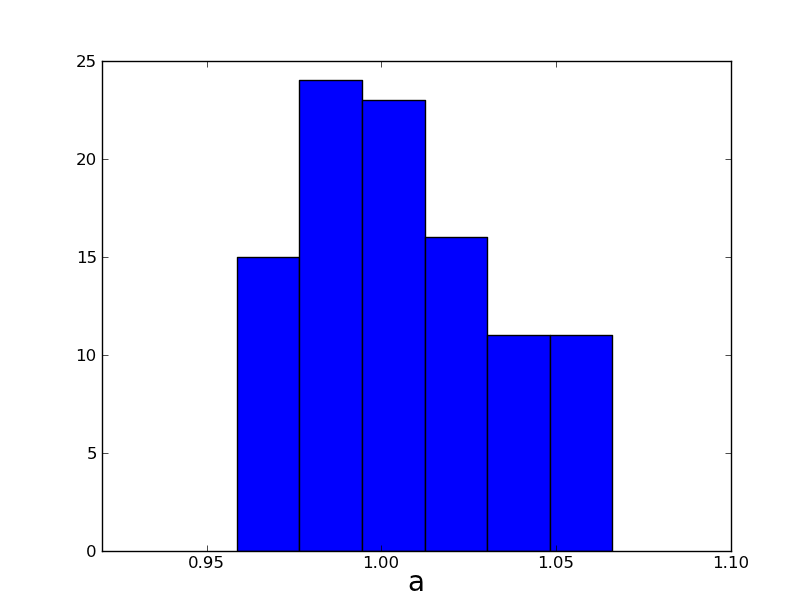
\includegraphics[width=0.5\linewidth]{smc_ad_hist_th1}} & \subfloat[]{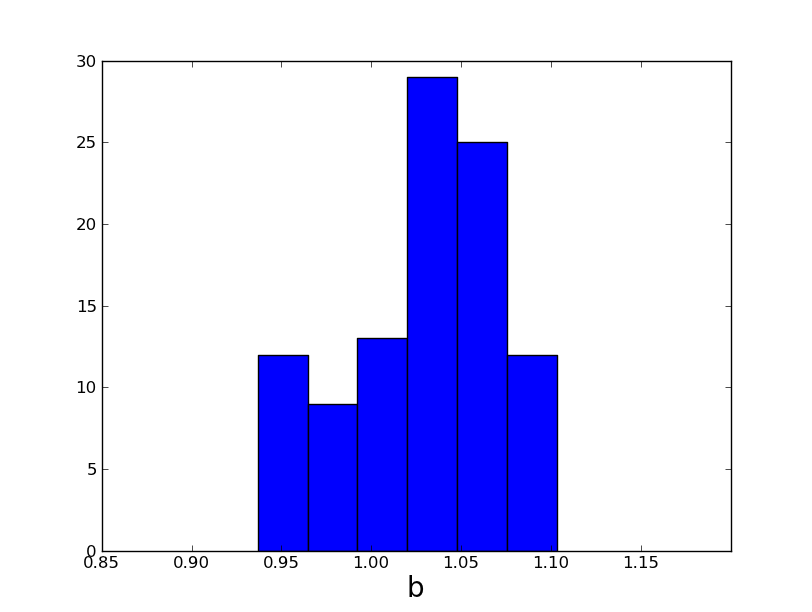
\includegraphics[width=0.5\linewidth]{smc_ad_hist_th2}}\\
\subfloat[]{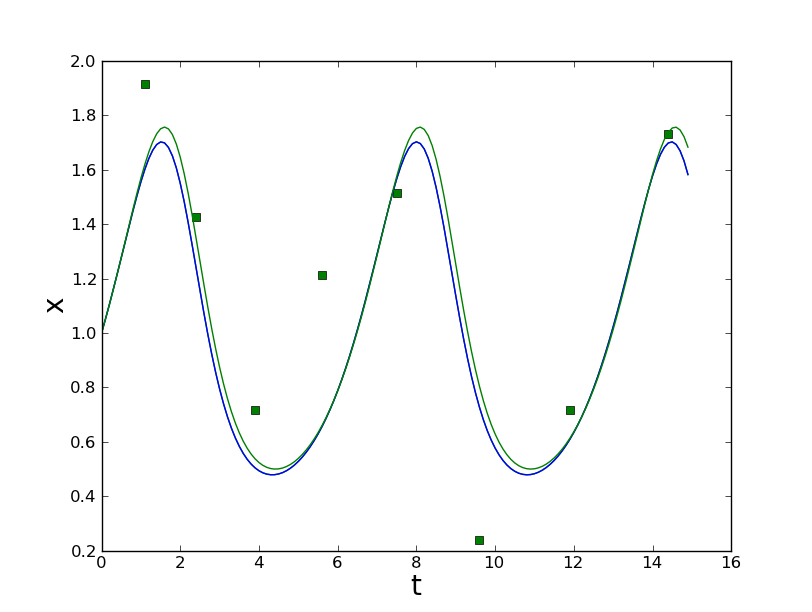
\includegraphics[width=0.5\linewidth]{smc_ad_x}} & \subfloat[]{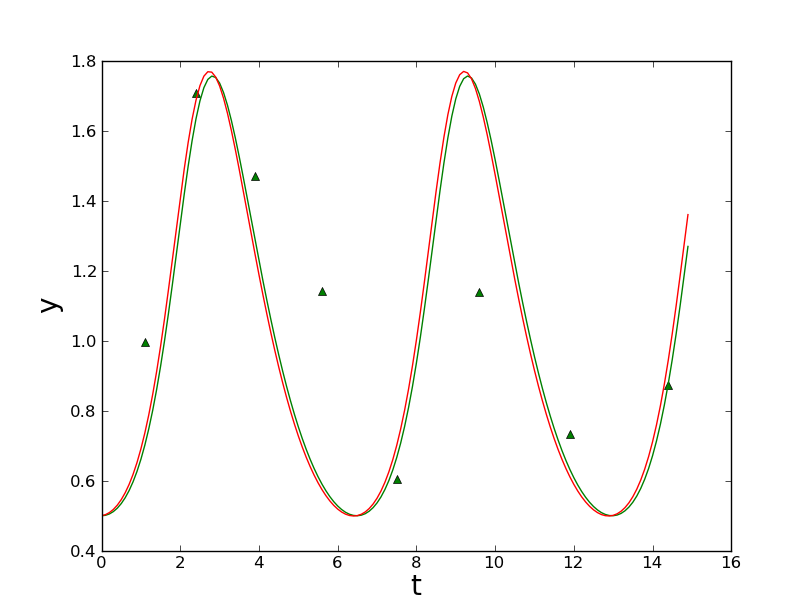
\includegraphics[width=0.5\linewidth]{smc_ad_y}}\\
\end{tabular}
\end{tabularx}
\caption{Inferred posteriors and quality of solution}\label{fig:smc_ad}
\end{figure}



% ------------------------------------------------------------------------

%%% Local Variables: 
%%% mode: latex
%%% TeX-master: "../thesis"
%%% End: 
